\section{Implementation}
We will now discuss the implementation of our algorithm. Here we will discuss how the robot will be simulated in software, and we will also discuss how the robot will use a genetic algorithm to train a neural network to navigate.
\subsection{Training}
The robot is trained using a genetic algorithm. This genetic algorithm will create a population of chromosomes, these will simply be a sequence of doubles representing the weights for our NN. The algorithm will then initialise a NN with each set of weights. Once created these NNs will be allowed to run through the scenario controlling the robot. Once the generation has completed all it's runs, the chromosomes will be ranked according to their performance in the scenario. After ranking the robots will be selected using a roulette wheel selection method. This will mean that stronger characteristics should be carried forward, however it may also pick up from weaker performing chromosomes too, which should preserve some diversity to prevent stagnation at a local minimum. The selected children will then be either passed through back to the next generation, or they will be mutated and crossed over, according to the mutation chance. These are then joined with the population where the weakest candidates are then removed. The process is then repeated until the end condition is met. Which is either a suitably fit candidate, e.g. does not collide; or a suitable number of generations has passed.
\subsection{Robot Control}
The robot will be able to move around a grid and able to choose to move forwards backwards left and right. It will also have visibility in these squares too.

These decisions as to where to move in the grid are formed by a neural network. The neural network has 4 inputs, which represent the content of the squares directly in front and behind, and to the left and right. From this the NN will create a single output of a value between 1 and 10. The output will then be used to determine which way to move as described in table \ref{tab:outputdirectoin}.

\begin{table}
\centering
	\begin{tabular}{|c|c|}
	\hline
	Direction & Output\\
	\hline
	Left & 0-2.5\\
	\hline
	Forward & 2.5-5\\
	\hline
	Right & 5-7.5\\
	\hline
	Backward & 7.5-10\\
	\hline
	\end{tabular}
	\caption{Output mapping to movement.}
	\label{tab:outputdirectoin}
\end{table}
\subsection{Simulator}
The simulation software is written in C\#. The robot will be simulated in a two dimensional grid shown in figure \ref{fig:trainingUI}. 

\begin{figure}[h]
	\centering
	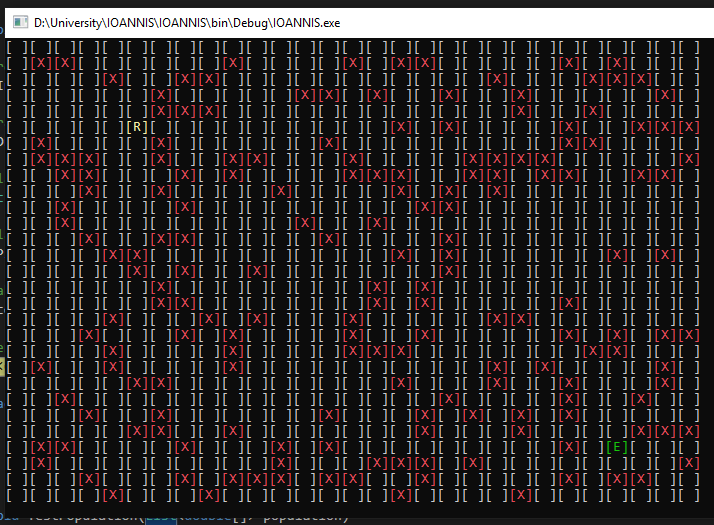
\includegraphics[width=0.9\linewidth]{ui1}
	\caption{Training UI.}
	\label{fig:trainingUI}
\end{figure}

In this grid the `X' symbol represents obstacles to be avoided, `R' represents the robot, and `E' represents the goal.